\documentclass[11pt]{article}
\usepackage[utf8]{inputenc}
\usepackage{amsmath}
\usepackage{amssymb}
\usepackage{geometry}
\usepackage{booktabs}
\usepackage{fancyhdr}
\usepackage{graphicx}
\usepackage{float}
\usepackage{listings}
\usepackage{listingsutf8}
\usepackage{xcolor}
\usepackage{titlesec}
\usepackage{adjustbox}
\usepackage{hyperref}

\titleformat{\section}{\normalfont\large\bfseries}{\thesection}{1em}{}
\titleformat{\subsection}{\normalfont\normalsize\bfseries}{\thesubsection}{1em}{}

\definecolor{codegreen}{rgb}{0,0.6,0}
\definecolor{codegray}{rgb}{0.5,0.5,0.5}
\definecolor{codepurple}{rgb}{0.58,0,0.82}
\definecolor{backcolour}{rgb}{0.95,0.95,0.92}

\lstdefinestyle{mystyle}{
  backgroundcolor=\color{backcolour},
  commentstyle=\color{codegreen},
  keywordstyle=\color{magenta},
  numberstyle=\tiny\color{codegray},
  stringstyle=\color{codepurple},
  basicstyle=\ttfamily\footnotesize,
  breakatwhitespace=false,
  breaklines=true,
  captionpos=b,
  keepspaces=true,
  numbers=left,
  numbersep=5pt,
  showspaces=false,
  showstringspaces=false,
  showtabs=false,
  tabsize=2
}
\lstset{style=mystyle}

\geometry{a4paper, margin=1in}
\setlength{\parindent}{0pt}
\setlength{\parskip}{0.5em}
\setlength{\headheight}{15pt}

\pagestyle{fancy}
\fancyhf{}
\lhead{Spring 2026 Intro to Deep Learning}
\rhead{Homework 4}
\rfoot{Page \thepage}

\begin{document}

\begin{center}
  {\Large \textbf{Modified LeNet-5 for CIFAR-10 Image Classification}} \\
  \vspace{0.2cm}
  {\large Homework Assignment 4} \\
  \vspace{0.2cm}
  \textbf{Course:} Spring 2026 Introduction to Deep Learning \\
  \textbf{Name:} Karim Smires \\
  \textbf{Due Date:} April 20, 2026
\end{center}
\hrule
\vspace{0.5cm}

\section*{Abstract}
This report presents a modified LeNet-5 implementation for CIFAR-10 colorful image
classification using PyTorch. Three network variants are evaluated: a baseline model
without Dropout or Batch Normalization, a model with an added Dropout layer, and a
model with Batch Normalization layers. All models are trained for 20 epochs using the
Adam optimizer and compared using training accuracy, test accuracy, and total training
time. The baseline model reaches 62.24\% test accuracy, the Dropout model improves
generalization to 64.34\%, and the Batch Normalization model performs best with
66.47\% test accuracy. All three models satisfy the assignment requirement of exceeding
50\% test accuracy, with Batch Normalization providing the strongest overall
improvement.

\section{Introduction}
The goal of this homework is to build and evaluate a modified LeNet-5 network for
CIFAR-10 image classification. Unlike the original LeNet-5, which was designed for
grayscale handwritten digits, CIFAR-10 contains small natural RGB images from ten
object categories. This makes the classification task more challenging and requires
adjusting the input layer from one channel to three channels.

In addition to implementing the baseline architecture, the assignment requires testing
two common regularization and stabilization techniques: Dropout and Batch
Normalization. These methods are widely used in deep learning because they can improve
generalization and training behavior. The purpose of this report is to describe the
three implemented models, summarize the training setup, and compare their performance
on CIFAR-10.

\section{Related Work}
\textbf{LeNet-5} \cite{lecun1998gradient} is one of the earliest successful convolutional
neural networks and was originally proposed for handwritten digit recognition. Its
stacked convolutional and fully connected design became a foundational architecture for
later CNN models.

\textbf{Dropout} \cite{srivastava2014dropout} is a regularization technique that randomly
deactivates a subset of neurons during training. This reduces co-adaptation between
features and often improves test performance by lowering overfitting.

\textbf{Batch Normalization} \cite{ioffe2015batch} normalizes intermediate activations
within a mini-batch and then applies learned scale and shift parameters. It often
stabilizes optimization, speeds convergence, and can provide a mild regularization
effect.

\section{Data Description}
The CIFAR-10 dataset consists of 60{,}000 color images of size $32 \times 32$ drawn
from ten object classes: airplane, automobile, bird, cat, deer, dog, frog, horse,
ship, and truck.

\begin{itemize}
  \item \textbf{Training set:} 50,000 images
  \item \textbf{Test set:} 10,000 images
  \item \textbf{Image shape:} $3 \times 32 \times 32$
  \item \textbf{Classes:} 10
\end{itemize}

Images are converted to tensors and normalized channel-wise using the standard
CIFAR-10 statistics implemented in the code:
\[
  \mu = (0.4914, 0.4822, 0.4465), \qquad
  \sigma = (0.2470, 0.2435, 0.2616)
\]
No data augmentation is used in this homework.

\section{Method Description}

\subsection{Baseline Model}
The baseline model is a modified LeNet-5 adapted to RGB input. It uses three
convolutional layers followed by two fully connected layers and ends with a
\texttt{LogSoftmax} output so that the model can be trained with negative log-likelihood
loss.

\subsection{Dropout Model}
The Dropout variant keeps the same convolutional structure as the baseline but inserts
one \texttt{nn.Dropout(p=0.5)} layer after the first fully connected layer. During
training, Dropout randomly zeroes activations with probability $p=0.5$, which helps
reduce overfitting by preventing the network from relying too heavily on particular
hidden units.

\subsection{Batch Normalization Model}
The Batch Normalization variant adds normalization layers after each convolutional
layer and after the first fully connected layer. The ordering used in the code is
Conv/Linear $\rightarrow$ BatchNorm $\rightarrow$ ReLU, which follows standard practice.
For a mini-batch input $x$, Batch Normalization computes
\[
  \hat{x} = \frac{x - \mu_{\mathcal{B}}}{\sqrt{\sigma_{\mathcal{B}}^2 + \epsilon}},
  \qquad
  y = \gamma \hat{x} + \beta
\]
where $\mu_{\mathcal{B}}$ and $\sigma_{\mathcal{B}}^2$ are the batch mean and variance,
while $\gamma$ and $\beta$ are learnable parameters.

\section{Model Description}

The implemented modified LeNet-5 architecture for CIFAR-10 is summarized below.

\begin{table}[H]
  \centering
  \begin{tabular}{llll}
    \toprule
    \textbf{Layer} & \textbf{Operation} & \textbf{Output Shape} & \textbf{Notes} \\
    \midrule
    Input   & ---                                & $3 \times 32 \times 32$ & RGB image \\
    C1      & Conv2d($3{\to}6$, $5 \times 5$)   & $6 \times 28 \times 28$ & [BN] $\to$ ReLU \\
    S2      & MaxPool2d($2 \times 2$)           & $6 \times 14 \times 14$ & \\
    C3      & Conv2d($6{\to}16$, $5 \times 5$)  & $16 \times 10 \times 10$ & [BN] $\to$ ReLU \\
    S4      & MaxPool2d($2 \times 2$)           & $16 \times 5 \times 5$ & \\
    C5      & Conv2d($16{\to}120$, $5 \times 5$)& $120 \times 1 \times 1$ & [BN] $\to$ ReLU \\
    Flatten & ---                               & $120$ & \\
    F6      & Linear($120{\to}84$)              & $84$ & [BN] $\to$ ReLU $\to$ [Dropout] \\
    F7      & Linear($84{\to}10$)               & $10$ & LogSoftmax output \\
    \bottomrule
  \end{tabular}
  \caption{Modified LeNet-5 architecture used in the homework. Bracketed layers are
  included only in the corresponding variant.}
\end{table}

The three evaluated configurations are:
\begin{enumerate}
  \item \textbf{Baseline:} no Dropout and no Batch Normalization.
  \item \textbf{Dropout:} one Dropout layer after F6.
  \item \textbf{BatchNorm:} BatchNorm layers after C1, C3, C5, and F6.
\end{enumerate}

\section{Experimental Procedure and Results}

\subsection{Experimental Setup}
All models are trained using the same training procedure so that the comparison is
fair.

\begin{table}[H]
  \centering
  \begin{tabular}{ll}
    \toprule
    \textbf{Hyperparameter} & \textbf{Value} \\
    \midrule
    Optimizer & Adam \\
    Learning rate & 0.001 \\
    Batch size & 64 \\
    Epochs & 20 \\
    Loss function & NLLLoss \\
    Dataset & CIFAR-10 \\
    \bottomrule
  \end{tabular}
  \caption{Shared hyperparameters used for all three models.}
\end{table}

During each epoch, training accuracy is computed from the mini-batches seen in the
training loop, and test accuracy is computed by evaluating the model on the full test
set. Total wall-clock training time is also recorded for each model.

\subsection{Results}

\begin{table}[H]
  \centering
  \begin{tabular}{lccc}
    \toprule
    \textbf{Model} & \textbf{Train Acc} & \textbf{Test Acc} & \textbf{Time} \\
    \midrule
    Baseline  & 76.67\% & 62.24\% & 65.1 s \\
    Dropout   & 72.02\% & 64.34\% & 65.0 s \\
    BatchNorm & \textbf{82.69\%} & \textbf{66.47\%} & 68.8 s \\
    \bottomrule
  \end{tabular}
  \caption{Final training accuracy, final test accuracy, and training time for the
  three model variants.}
\end{table}

\begin{figure}[H]
  \centering
  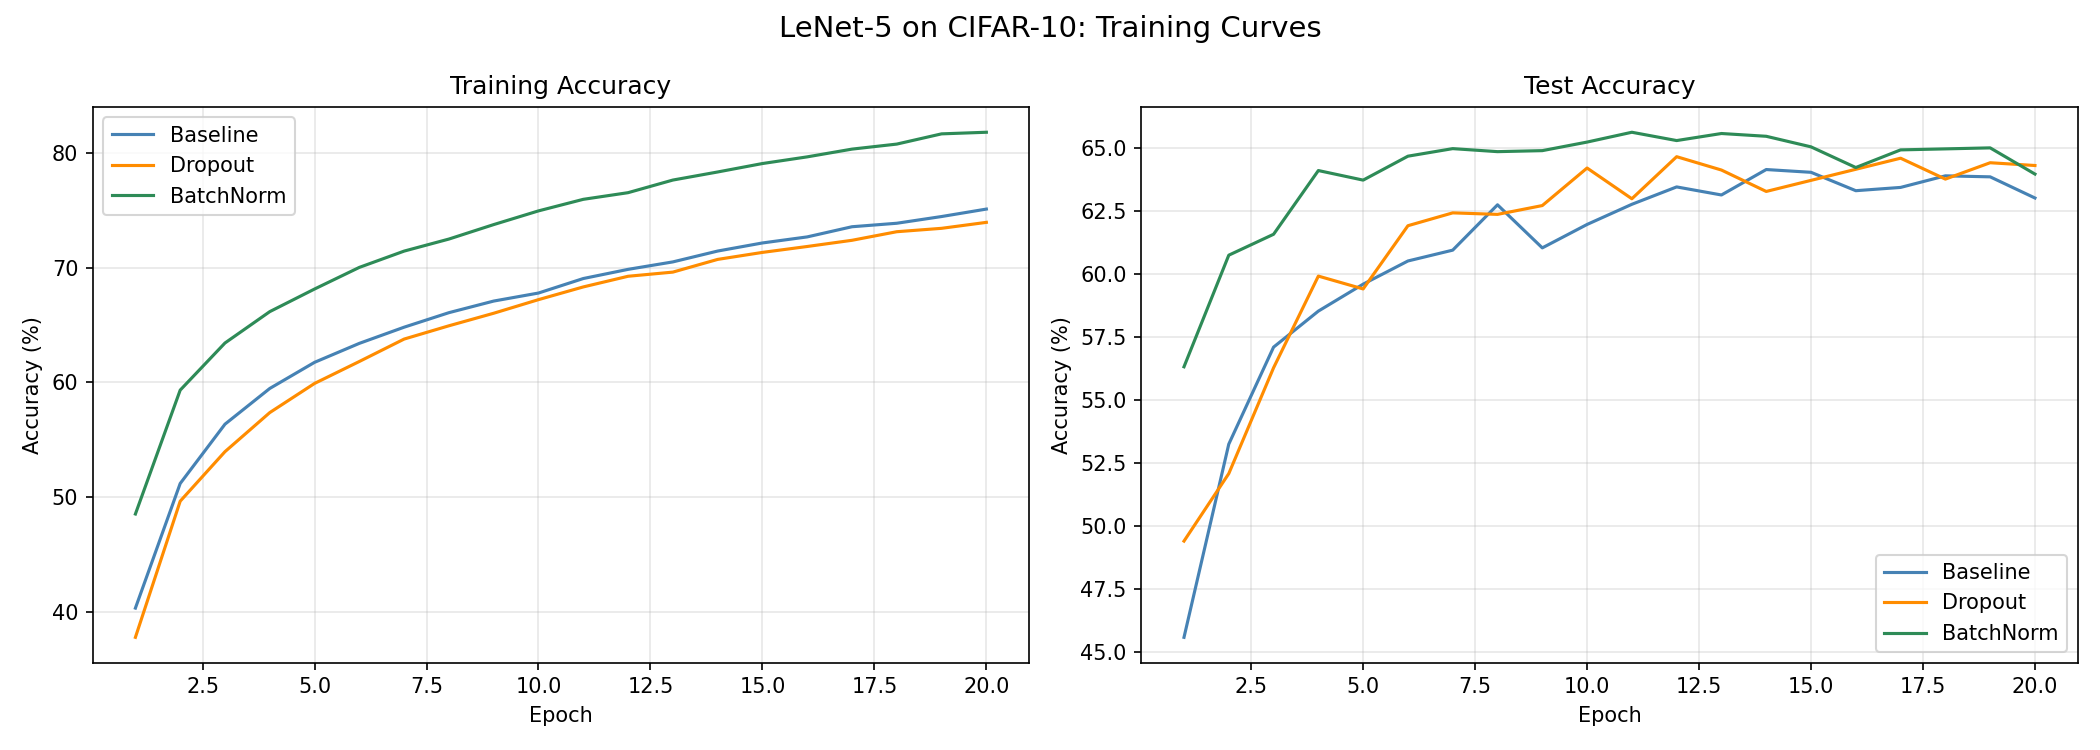
\includegraphics[width=\textwidth]{training_curves.png}
  \caption{Training accuracy and test accuracy curves for the three LeNet-5 variants on
  CIFAR-10.}
  \label{fig:training_curves}
\end{figure}

\subsection{Analysis}
All three models exceed the assignment requirement of 50\% test accuracy, which shows
that the modified LeNet-5 architecture is sufficient to learn useful features on
CIFAR-10.

\textbf{Baseline performance.} The baseline model achieves 62.24\% test accuracy with
76.67\% training accuracy. The gap between train and test accuracy suggests moderate
overfitting as training progresses.

\textbf{Effect of Dropout.} Adding one Dropout layer decreases the final training
accuracy to 72.02\% but improves the test accuracy to 64.34\%. This is the expected
pattern for regularization: the model fits the training data less aggressively while
generalizing better to unseen data.

\textbf{Effect of Batch Normalization.} The BatchNorm model achieves the best overall
performance, reaching 82.69\% training accuracy and 66.47\% test accuracy. It also
shows faster early convergence in the recorded results. This suggests that Batch
Normalization improves optimization and allows the network to learn stronger features
without sacrificing generalization.

\textbf{Overall comparison.} Among the three variants, Batch Normalization provides the
largest performance gain over the baseline, improving test accuracy by 4.23 percentage
points. Dropout also improves generalization, but its gain is smaller at 2.10
percentage points. Based on these results, Batch Normalization is the most effective
modification for this homework setting.

\section{Conclusion}
This homework implemented and evaluated three modified LeNet-5 models for CIFAR-10
classification. The baseline model provided a solid starting point and already exceeded
the required 50\% test accuracy. Adding Dropout improved generalization, while adding
Batch Normalization produced the best overall result.

The final ranking is:
\begin{enumerate}
  \item \textbf{BatchNorm}: 66.47\% test accuracy
  \item \textbf{Dropout}: 64.34\% test accuracy
  \item \textbf{Baseline}: 62.24\% test accuracy
\end{enumerate}

These results show that both regularization and normalization are useful for LeNet-5 on
CIFAR-10, with Batch Normalization offering the strongest benefit in this experiment.

\begin{thebibliography}{9}

\bibitem{lecun1998gradient}
Y. LeCun, L. Bottou, Y. Bengio, and P. Haffner,
``Gradient-based learning applied to document recognition,''
\textit{Proceedings of the IEEE}, vol.\ 86, no.\ 11, pp.\ 2278--2324, 1998.

\bibitem{srivastava2014dropout}
N. Srivastava, G. Hinton, A. Krizhevsky, I. Sutskever, and R. Salakhutdinov,
``Dropout: A simple way to prevent neural networks from overfitting,''
\textit{Journal of Machine Learning Research}, vol.\ 15, pp.\ 1929--1958, 2014.

\bibitem{ioffe2015batch}
S. Ioffe and C. Szegedy,
``Batch normalization: Accelerating deep network training by reducing internal covariate shift,''
in \textit{Proc.\ International Conference on Machine Learning (ICML)}, pp.\ 448--456, 2015.

\end{thebibliography}

\vspace{0.5cm}
\hrule
\vspace{0.5cm}

\appendix
\section{Source Code}

\lstinputlisting[
  language=Python,
  inputencoding=utf8/latin1,
  caption=hw4.py --- modified LeNet-5 training and evaluation
]{hw4.py}

\end{document}
